\section{Electronics}
% In this section briefly describe the software and hardware of the robot
\setlength\intextsep{0pt}
Last year there were major changes applied to the design of the electronics. At the time of writing this paper, it has been about one year which these circuits were used and have been tested and qualified in different matches. Currently all the robots (including the 3D-printed robots) are functioning with the help of these circuits. The reader is referred to the previous years TDP [1]of this team for more details about the main circuit.\\
\indent For this year, (1)There have been some research made for designing the teams future sender base in order to communicate with a great number of robots. (2)A new type of motor encoder is used for a better and more reliable robot navigation.

\subsection{Communication}
Last year, teams in division A were permitted to use 8 robots in the field during the play, in the next years this limit will increase to 11. This fact comes with different challenges for all teams related to there robots communication system.\\
\indent Number of links to every robot from a senders base, bit rate and packet size limit are the three parameters that have an inverse relationship with each other. Some teams solve this problem by using two or more sender bases, each controlling a set of robots. A few other teams decided to send there data with a lower rate or smaller packet size. In the Immortals team the goal was to use a single sender base without reducing neither the three parameters. Using the same type of RF module on the main circuit of the robot [2]. Currently the sender which is used to communicate with the robots, is using a RF module called the NRF24L01 from Nordic Co., The RF module implemented on the robot is NRF52832 which also is from Nordic Co.. Both the modules are capable of using the Enhanced ShockBurst protocol (ESB) and are currently using that protocol to communicate. The NRF24l01 acts as a bottle neck for the system since it has a slower bit rate in compare to the NRF52832 Thus, it is decided to design a sender base with the NRF52832.\\
\indent By using an nRF52 Development Board and an Arduino Ethernet Shield it is possible to setup a simple sender base equipped with the NRF52832 module (see Fig. \ref{fig:SIMPLE_SENDER}).\\
\begin{figure}
	\centering
	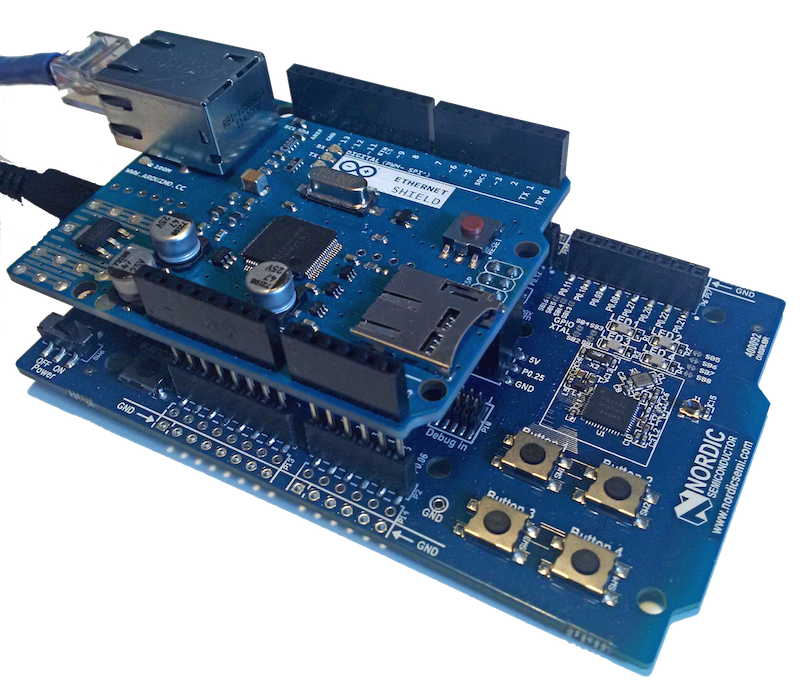
\includegraphics[width=0.6\textwidth]{images/NRF52832DK_ETH.png}
	\caption{A sender made by deploying an Arduino Ethernet Shield on a nRF52 DK board}
	\label{fig:SIMPLE_SENDER}
\end{figure}\\
\indent After running many tests the average amount of packet loss for the link between the sender and the robot was negligible (less than one packet loss among 60 packets per second in average). Using the previous sender of the team (NRF24l01)the average packet loss was more than one out of 60 packets. Although this might not be a concern when the robots can still get navigated properly with a few packets lost, it may be important for teams that wish to run 11 robots in the future.\\

\subsection{Magnetic Encoder}
Until last year the robots were equipped with a disk encoder which required the motor to have a back shaft, If the backshaft bends slightly due to very hard collisions made with the wheel, the disk encoder will malfunction and in extreme cases the encoders disk and ciruit will hit each other resulting in the damege of the encoder itself.\\
\indent It was decided to use magnetic encoders due to the explained issues. The type of encoder which the team currently uses is TLE5012B-E1000 [5], The previous disk encoders were the E4T-500 Miniature Optical Kit Encoderers [6].\\
\indent After using the magnetic encoder the precision of the motor speed increased due to the high resolution of the magnetic encoders, there were no robot substitutions due to malfunctioning encoders, the process of assembling and disassembling a robot got very fast and easy, the motors we used were not needed to be specially customized which takes much time to get prepared by the manufacturer.\\
\indent On the other side the megnetic encoder outputs are a little vulnerable to noise and the data gets invalid when a strong magnetic field gets presented, For example when the robot performs a kick the encoders will give an invalid data output for a few tens of milliseconds.\\


%\begin{table}
%\center
%\begin{tabular}{| p{3cm} | p{3cm} | p{3cm} |}
%  \hline
%  - & E4T-500 & TLE5012B-E1000\\
%  \hline
%  \hline
%  resolution & 500 & 4096\\
%  \hline
%  salam & omg & omgwe\\
%  \hline
%\end{tabular}
%\caption{My table}
%\label{table:MAG_ENC}
%\end{table}


\begin{figure}
	\centering
	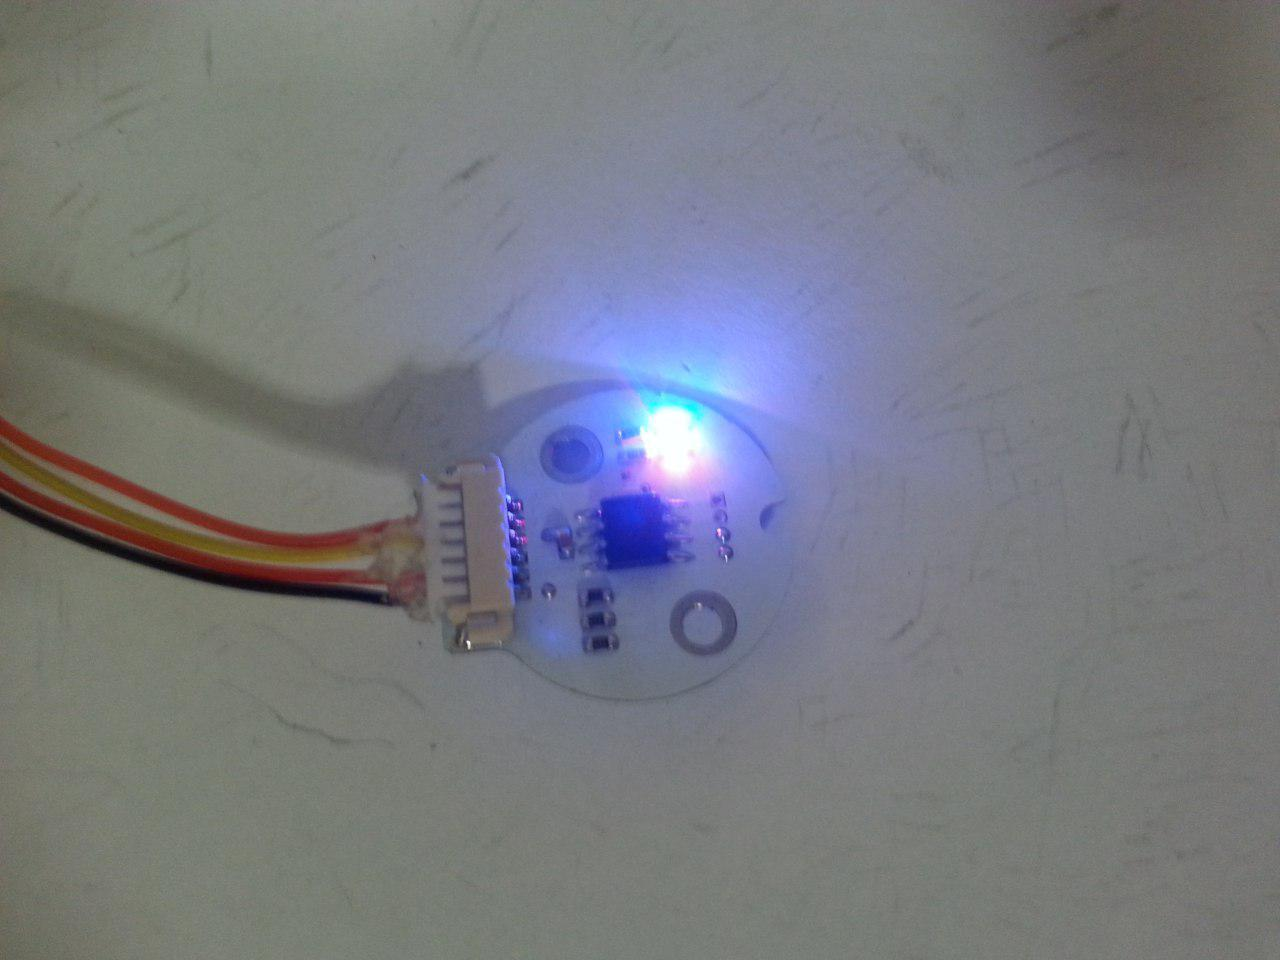
\includegraphics[width=0.6\textwidth]{images/MAG_ENC.jpg}
	\caption{Magnetic Encoder}
	\label{fig:MAG_ENC}
\end{figure}\\


%\begin{figure}
%	\centering
%	\includegraphics[width=0.4\textwidth]{images/wall-e.jpg}
%	\caption{Robot WALL-E}
%	\label{fig:wall-e}
%\end{figure}
%
%Robot WALL-E has the patented \textit{\BnL Optimized Design} for garbage recollection. Specifications are as follows:
%
%\begin{itemize}
%	\item Base: \BnL all-terrain base (differential pair), 2.5m/s max speed.
%	\item Torso: \BnL compressor with solar charger.
%	\item Left and right arms: Mounted on torso. \BnL 7DOF, anthropomorphic. Maximum load: 20kg.
%	\item Neck: \BnL telescopic neck with pan and tilt.
%	\item Head: 3DOF \BnL Expressive Eyes
%	\item Robot dimensions: height: 1.2m (max), width: 0.7m depth 0.8m
%	\item Robot weight: 50kg.
%\end{itemize}
%
%\noindent\textit{Also our robot incorporates the following devices:}
%
%\begin{itemize}
%	\item \BnL Battery charge indicator
%	\item \BnL Auto-focus all-purpose cameras
%	\item \BnL 7DOF heavy duty fingers
%	\item \BnL Cockroach
%\end{itemize}
%
%\section*{Robot's Software Description}
%% Please describe in this section the software you are using to control your robot. Consider the following example:
%
%\textit{For our robot we are using the following software:}
%
%\begin{itemize}
%	\item Platform: \BnL Operating System
%	\item Navigation: \BnL Navigator
%	\item Face recognition: None. Not designed for human interaction.
%	\item Speech recognition: \BnL All-purpose recognizer \cite{bnl1}.
%	\item Speech generation: None. Not designed for human interaction.
%	\item Object recognition: \BnL Trash Seeker Algorithm (See previous sections).
%	\item Arms control and two-hand coordination: \BnL automatic controller \cite{bnl2}.
%\end{itemize}
%
%\section*{External Devices}
%% Please describe in this section the external devices used by your robot. Consider the following example:
%
%\textit{WALL-E robot relies on the following external hardware:}
%
%\begin{itemize}
%	\item \BnL Garbage Compactor
%	\item \BnL EVA unit
%	\item \BnL Data Cluster
%	\item $3 \times$ \BnL Ultra-Power laptops.
%\end{itemize}
%
%\section*{Cloud Services}
%% Please describe in this section the Cloud Services and online software used by your robot. Consider the following example:
%
%\textit{WALL-E connects the following cloud services:}
%\begin{itemize}
%	\item Localization and mapping: \BnL Geolocalization system \cite{bnl3}.
%\end{itemize}